\graphicspath{{Images/}}

\section{Preliminary Investigation}

\subsection{Types of Mesons}
The meson can be categorized into five types based on its spin and parity. As shown in the table below:

\begin{table}[htbp]
    \centering
    \caption{Types of Mesons}
    \vspace{4mm}
    \begin{tabular}{c | c c c c c}
        \hline \hline
        \textbf{Type of Meson} & \textbf{S} & \textbf{L} & \textbf{P} & \textbf{J} & \textbf{J$^{\textbf{P}}$} \\
        \hline
        Pseudoscalar Meson     & 0          & 0          & -          & 0          & 0-                        \\
        \hline
        Pseudovector Meson     & 0, 1       & 1          & +          & 1          & 1+                        \\
        \hline
        Vector Meson           & 1          & 0, 2       & -          & 1          & 1-                        \\
        \hline
        Scalar Meson           & 1          & 1          & +          & 0          & 0+                        \\
        \hline
        Tensor Meson           & 1          & 1, 3       & +          & 2          & 2+                        \\
        \hline\hline
    \end{tabular}
    \label{tab:mesons}
\end{table}


The quark composition of the $D_{s}^{+}$ meson is $c\bar{s}$ while the $D_{s}^{-}$ meson has a quark composition of $\bar{c}s$. The $\eta$ and $\eta^{\prime}$ mesons are isosinglet mesons made of a mixture of up, down, and strange quarks and their antiquarks. The basic SU(3) symmetry theory of quarks for the three lightest quarks, which only takes into account the strong force, predicts corresponding particles
\begin{equation}
    \eta_1=\frac{1}{\sqrt{3}}(\mathrm{u} \overline{\mathrm{u}}+\mathrm{d} \overline{\mathrm{d}}+\mathrm{s} \overline{\mathrm{s}})
\end{equation}
and
\begin{equation}
    \eta_8=\frac{1}{\sqrt{6}}(\mathrm{u} \overline{\mathrm{u}}+\mathrm{d} \overline{\mathrm{d}}-2 \mathrm{~s} \overline{\mathrm{s}})
\end{equation}
However, the electroweak interaction - which can transform one flavor of quark into another - causes a small but significant amount of "mixing" of the eigenstates (with mixing angle $\theta_{\mathrm{P}}$), so that the actual quark composition is a linear combination of these formulae. That is:
\begin{equation}
    \left(\begin{array}{cr}
        \cos \theta_{\mathrm{P}} & -\sin \theta_{\mathrm{P}} \\
        \sin \theta_{\mathrm{P}} & \cos \theta_{\mathrm{P}}
    \end{array}\right)\left(\begin{array}{l}
        \eta_8 \\
        \eta_1
    \end{array}\right)=\left(\begin{array}{c}
        \eta \\
        \eta^{\prime}
    \end{array}\right)
\end{equation}
The unsubscripted name $\eta$ refers to the real particle that is actually observed and close to the $\eta_8$. The $\eta^{\prime}$ is the observed particle close to $\eta_1$. Both $D_{s}^{+}$ and $\eta^{(\prime)}$ are pseudoscalar mesons.



\subsection{Decay process}
The process from \( D_{s}^{+} \) to \( \eta^{(\prime)} \ell \nu \) involves both strong and weak interactions. The Feynman diagram is shown in the figure below.


\begin{figure}[!hpt]\centering
    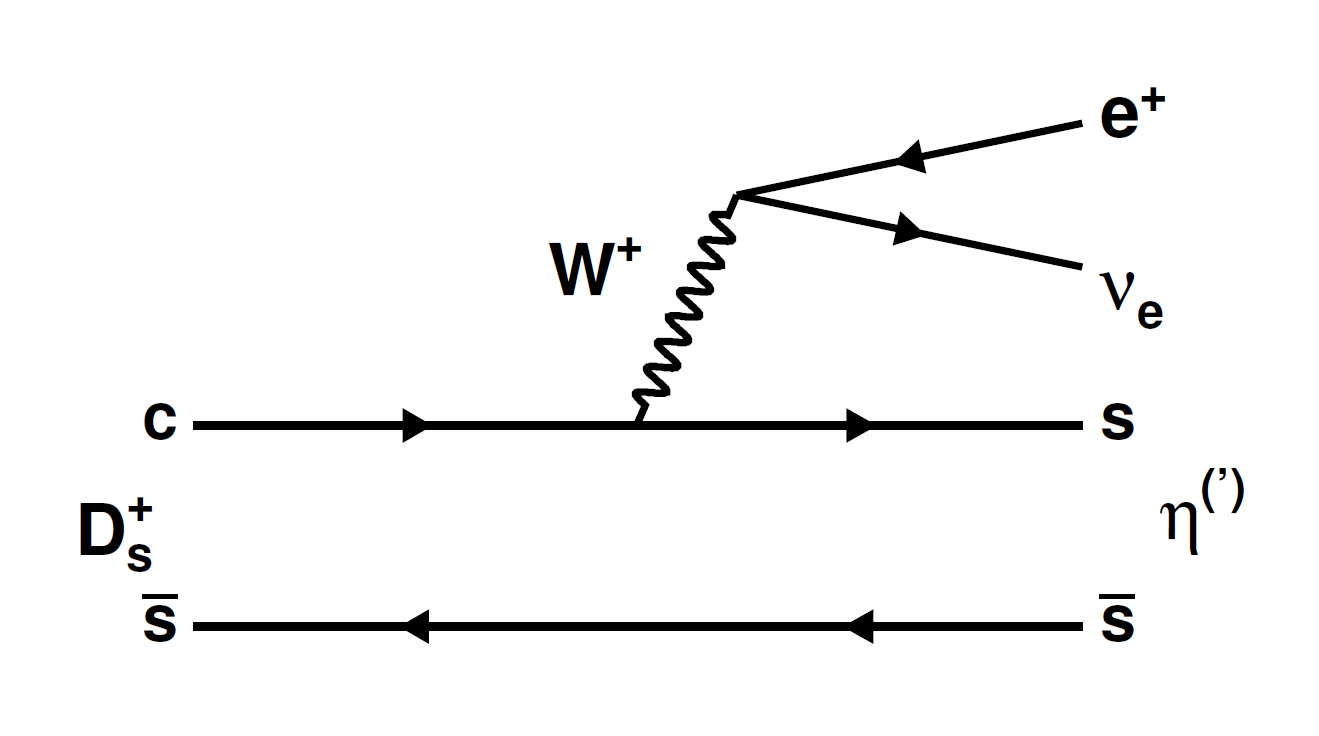
\includegraphics[width=0.5\textwidth]{image/diagram.png}
    \caption{The dominant Feynman diagram.}
    \label{fig:diagram1}
\end{figure}


